\subsection{Bandpass Changes due to Atmosphere}

\paragraph{Description:}
Atmospheric variables including precipitable water vapor (PWV), observing angle, and ground temperature can have significant effects on telescope observing conditions when making measurements of the Cosmic Microwave Background radiation.  More specifically, changes in the opacity of the atmosphere lead to variations in the effective gain of the instrument's bandpass.  Furthermore, these changes in opacity are frequency dependent, which lead to shifts in the central frequency of the instrument's bandpass.  Both band gain and central frequency are important factors in the data-to-map analysis pipeline, and any uncertainties in these values must be well understood.

\paragraph{Plan to model and/or measure:}
In order to model the effect of atmospheric changes on detector bandpasses, we first need to model the transmission of the atmosphere across the frequencies of interest.  This is accomplished by using the am Atmospheric Model code developed by Scott Paine from the Harvard-Smithsonian Center for Astrophysics.  The code comes equipped with various templates, one of which being the Chajnantor Plateau in Chile where the Simons Observatory will be located.  Several environmental parameters can be adjusted such as precipitable water vapor (PWV), zenith angle, and ground temperature.  The output of the code gives the transmission of the atmosphere vs frequency.  Figure \ref{transmissions} shows the plotted output for varying the PWV at a fixed ground temperature and zenith angle.   

Figure \ref{transmissions} also shows the average bandpasses for Advanced ACTPol 20, 40, 90, 150, and 220 GHz detectors.  With models of the bandpass, atmosphere transmission, and estimated spectrums of what we plan to observe (CMB, dust, etc.), we can then quantify variations in the band gain and centers caused by changing atmospheric conditions.

\begin{figure}[h] %  figure placement: here, top, bottom, or page
   \centering
   \centerline{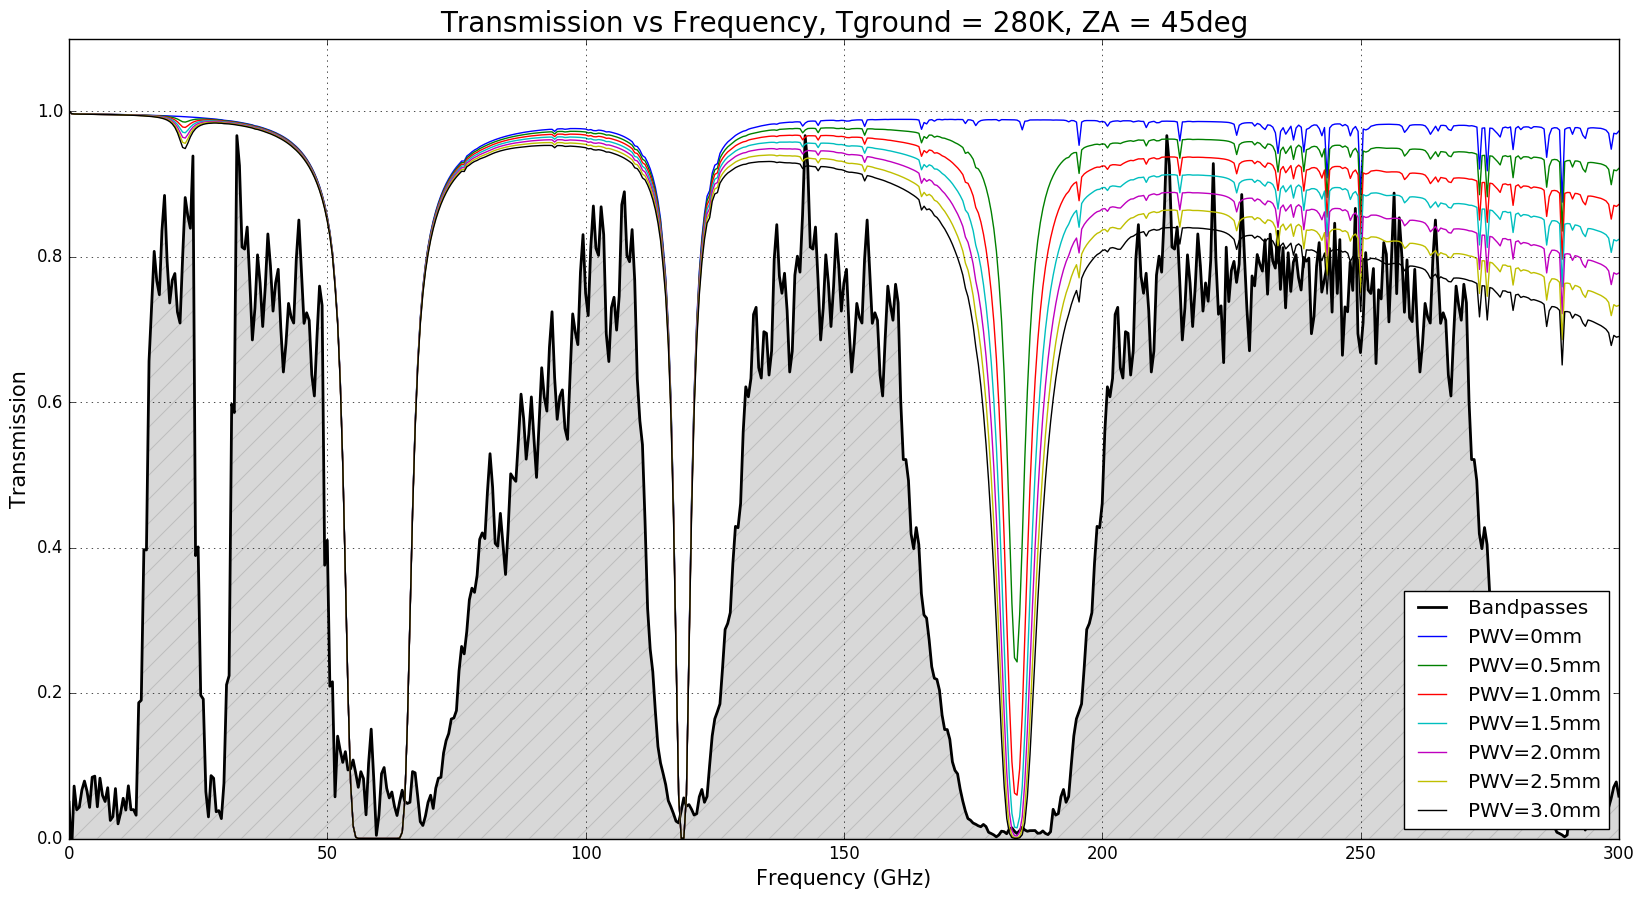
\includegraphics[width=\linewidth]{test.png}} 
   \caption{Atmosphere transmission lines and averaged bandpass for 20, 40, 90, 150, and 220 GHz channels.  A colored transmission line is plotted for each value of PWV while holding the observing angle and ground temperature constant.}
   \label{transmissions}
\end{figure}

To mitigate this effect, we have to have a good understanding of what our bandpasses look like from FTS measurements and what the atmosphere looks like. Improved FTS measurements compared to previous experiments are necessary mitigate this effetc and thus reach our science goals, especially at low~$\ell$. An on-site radiometer would also help by providing improved measurements of the atmosphere at the site, which would improve our atmospheric modeling. This effect has been modeled, but it is a design driver for calibration equipment, which will need to be improved for SO and S4 science goals. Thus, its SRF is a 5.

\paragraph{Uncertainty/Range:}
To calculate the changes in band due to atmospheric variations, the average bandpasses are multiplied by the atmosphere transmission lines.  We then compute the integrated power and central frequency of each of the five bands for each case.  For total atmosphere effects, the three parameters of PWV, ground temperature, and observing angle are combined together to estimate the minimum (smallest change to FTS measured band) and maximum (largest change to FTS measured band) observing conditions experienced during data collection.  The minimum change parameters are defined to be PWV = $0$mm, Tground = $290$K, and ZA = $30$deg and the maximum change parameters to be PWV = $3$mm,Tground = $250$K, and ZA = $60$deg.  These values correspond to the best and worst possible atmospheric conditions in useable data throughout a full observing season.  For example, data where PWV > 3mm is automatically discarded in the ACT science analysis.  Figure \ref{minmax_bands} shows the resulting bands for the minimum and maximum cases described above.  

The bands also change depending on the spectrum of the observed source.  In addition to simulating changes in the measured detector band alone, the band gain and band centers are also calculated for the detector bands multiplied by the CMB spectrum and the detector bands multiplied by an estimated dust spectrum $(\nu^{2.9})$.  It is important to test the changes for each observed source to identify whether or not the same calibrations can be used for all sources.  The top row in Figure \ref{minmax_bands} shows the minimum and maximum band changes for the measured band alone, the middle row shows the changes for an estimated dust spectrum, and the bottom row shows the changes for the CMB spectrum.

\textbf{Need a description on what constraints this places on FTS calibration in order to reach our science goals. Maybe a plot or two. Should also reference Jon Ward's upcoming paper (add to references and cite here).}

\begin{figure}[H]
\centering
 \begin{varwidth}{\linewidth}
 \subfloat{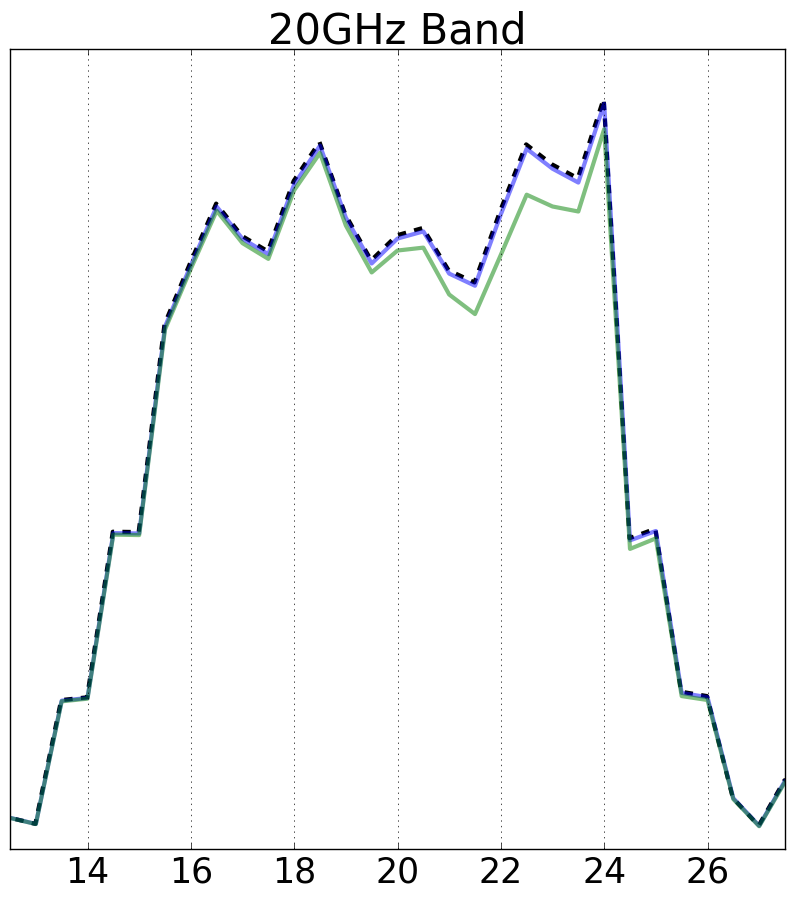
\includegraphics[width=.2\linewidth]{minmax_totals_20GHz.png}}
 \hspace{-2.5mm}
 \subfloat{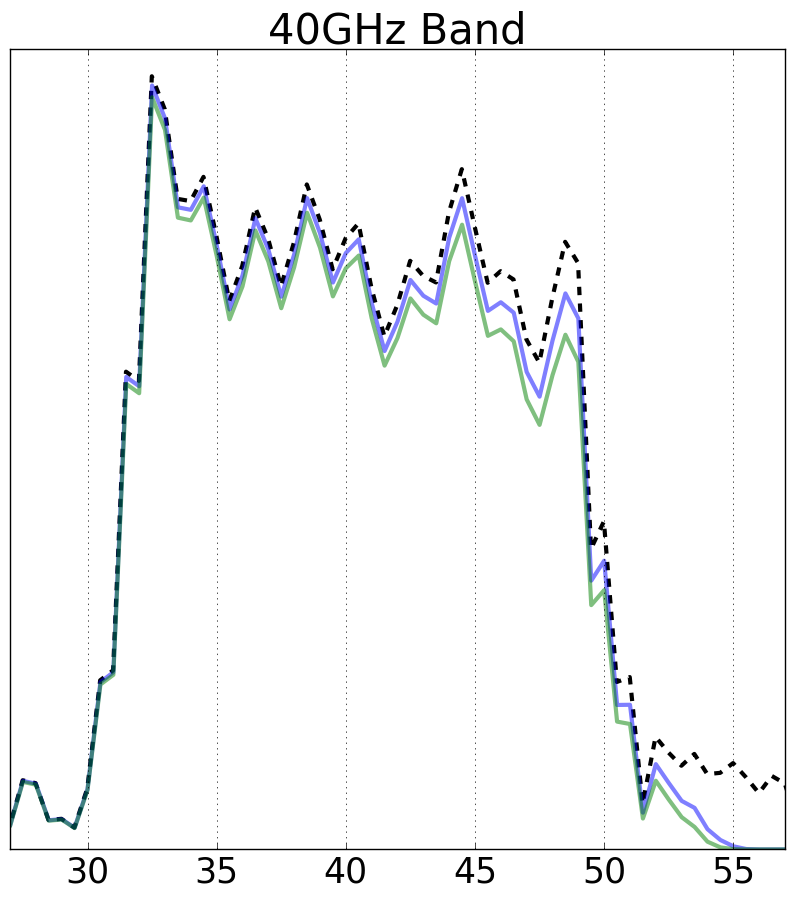
\includegraphics[width=.2\linewidth]{minmax_totals_40GHz.png}}
 \hspace{-2.5mm}
 \subfloat{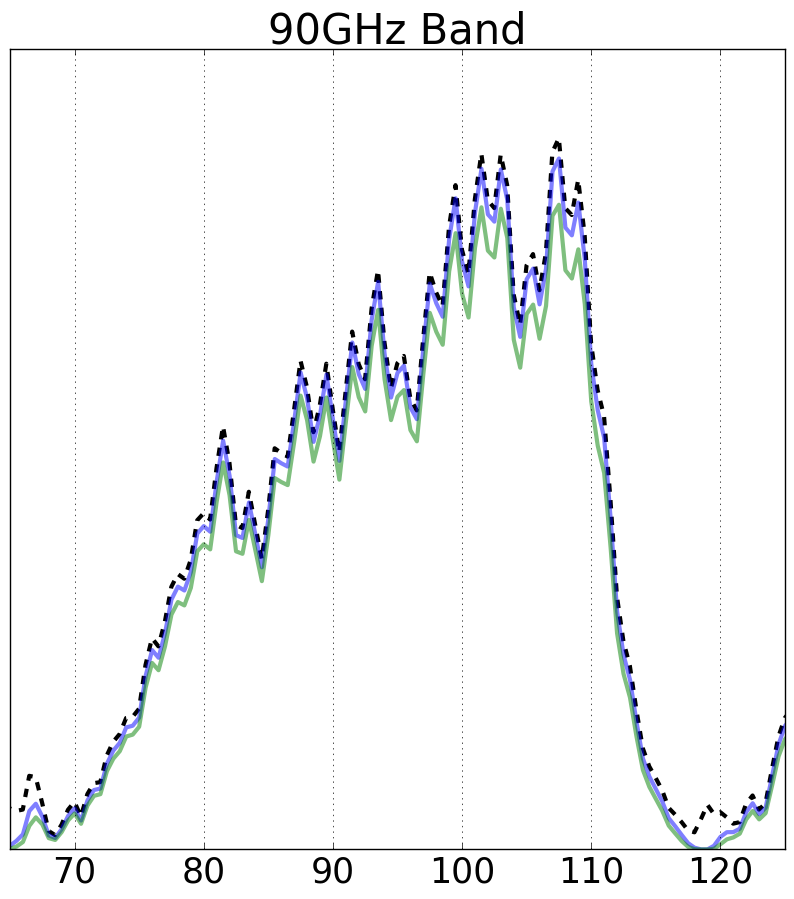
\includegraphics[width=.2\linewidth]{minmax_totals_90GHz.png}}
 \hspace{-2.5mm}
 \subfloat{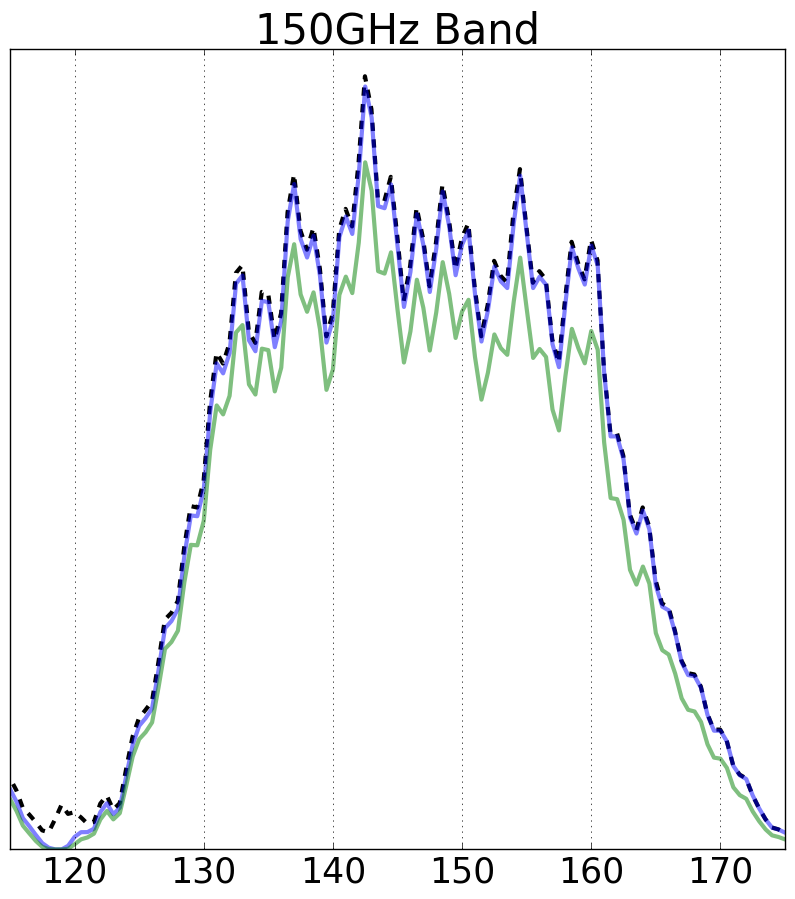
\includegraphics[width=.2\linewidth]{minmax_totals_150GHz.png}}
 \hspace{-2.5mm}
 \subfloat{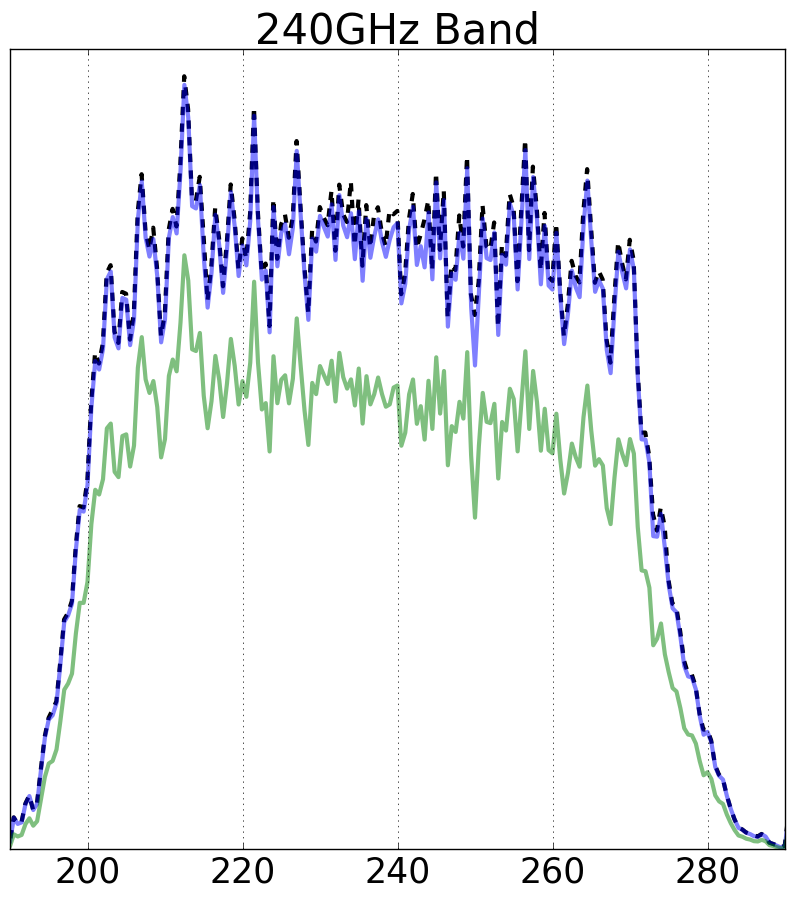
\includegraphics[width=.2\linewidth]{minmax_totals_240GHz.png}}
 \end{varwidth}
 \begin{varwidth}{\linewidth}
 \subfloat{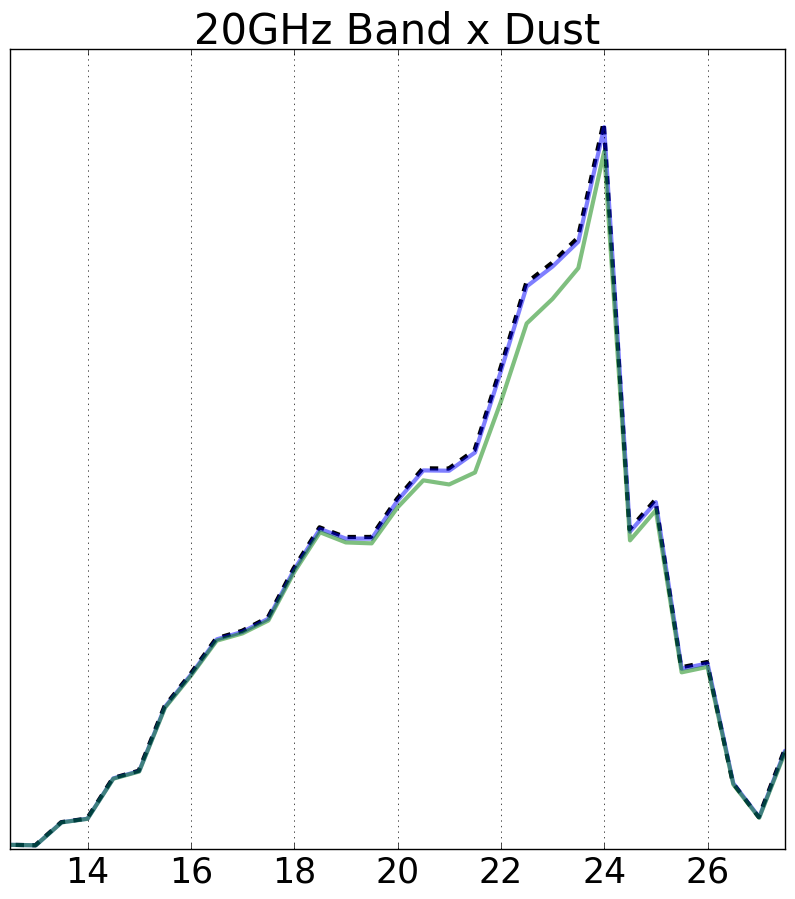
\includegraphics[width=.2\linewidth]{minmax_totals_20GHz_dust.png}}
 \hspace{-2.5mm}
 \subfloat{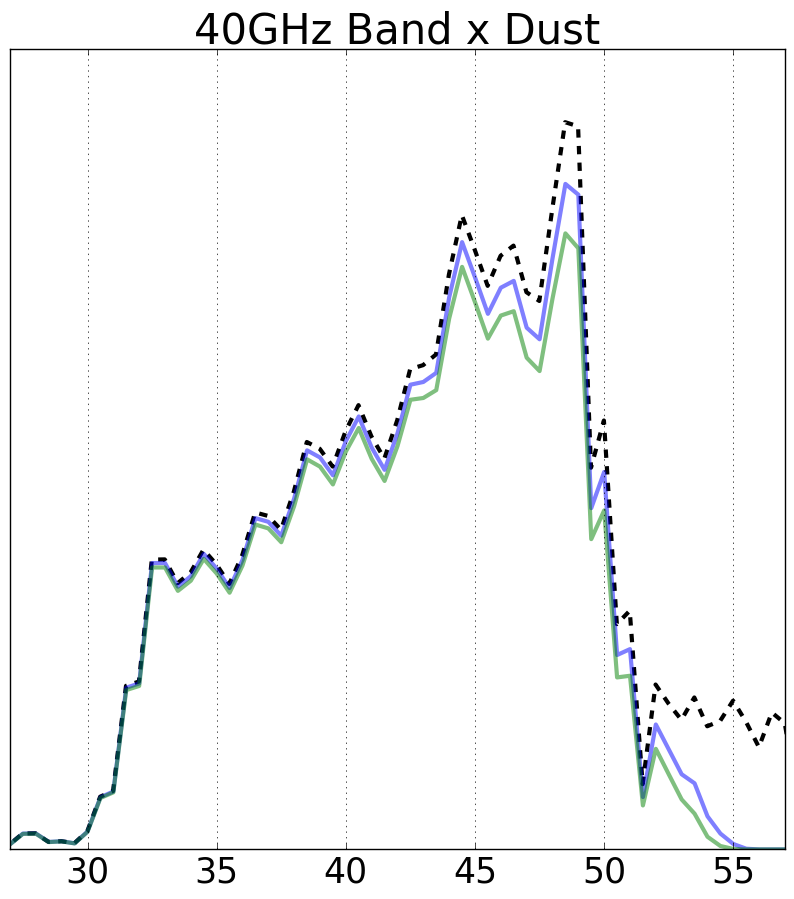
\includegraphics[width=.2\linewidth]{minmax_totals_40GHz_dust.png}}
 \hspace{-2.5mm}
 \subfloat{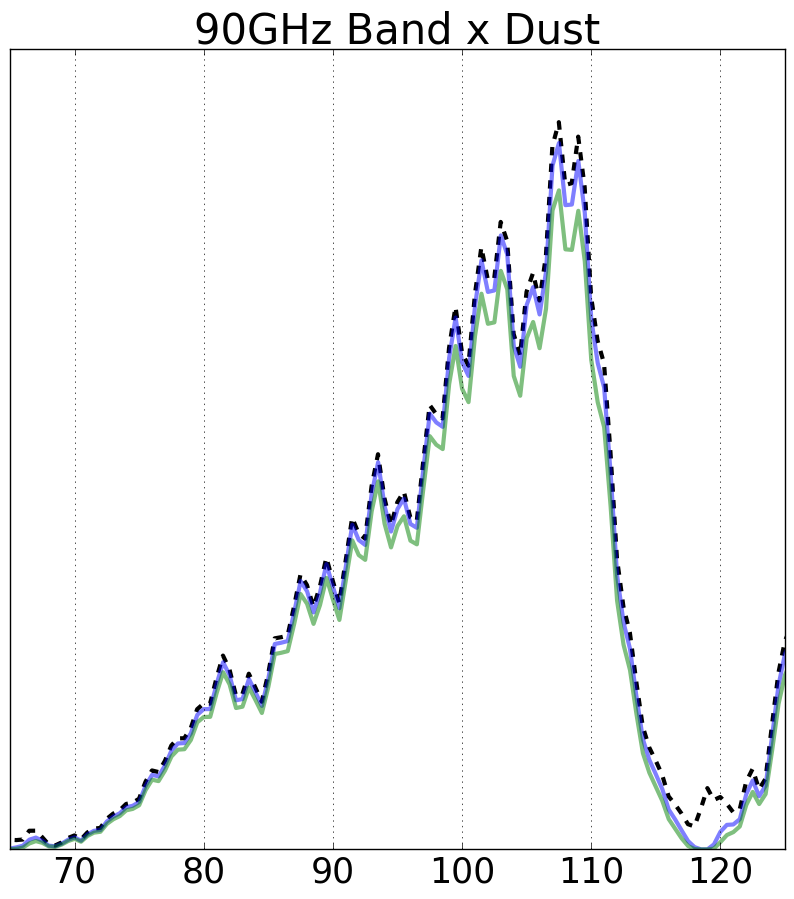
\includegraphics[width=.2\linewidth]{minmax_totals_90GHz_dust.png}}
 \hspace{-2.5mm}
 \subfloat{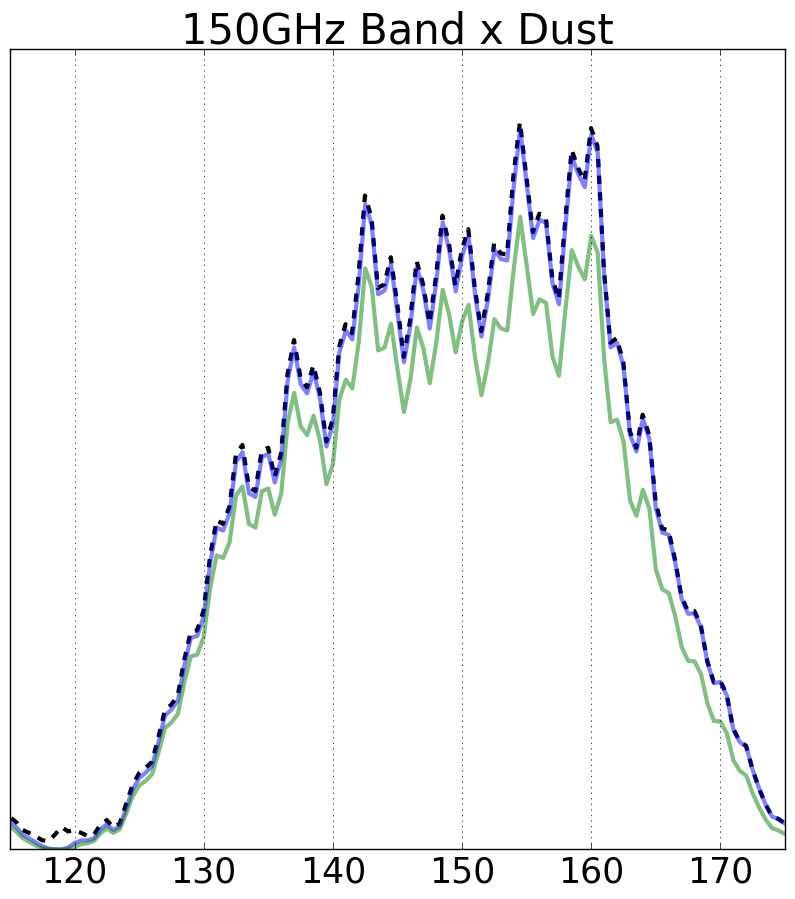
\includegraphics[width=.2\linewidth]{minmax_totals_150GHz_dust.png}}
 \hspace{-2.5mm}
 \subfloat{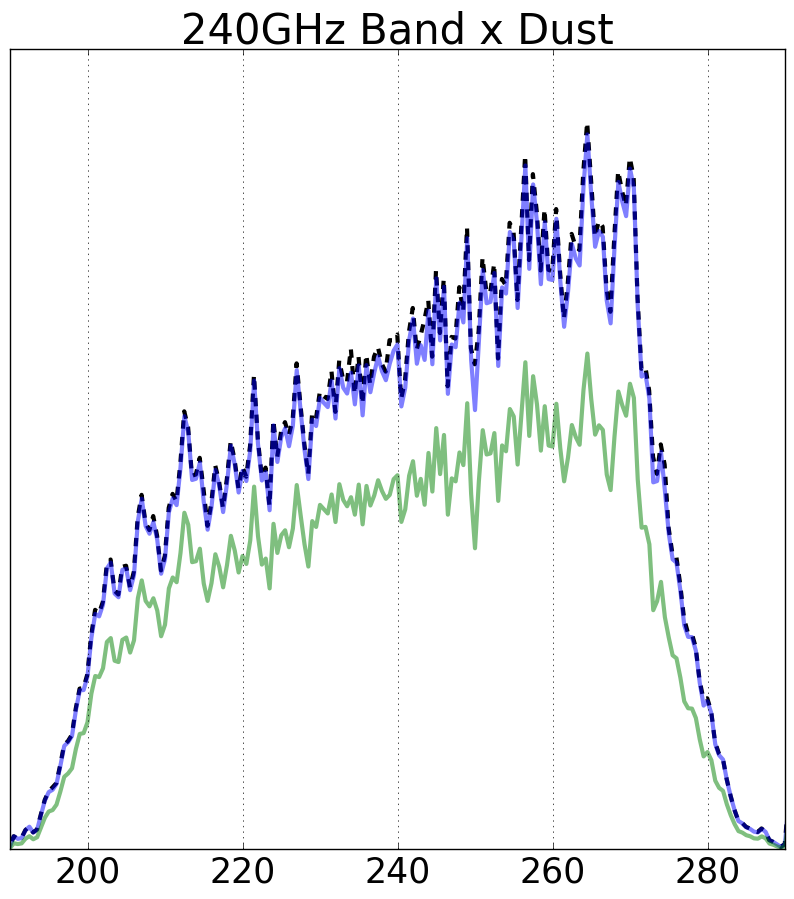
\includegraphics[width=.2\linewidth]{minmax_totals_240GHz_dust.png}}
 \end{varwidth}
 \begin{varwidth}{\linewidth}
 \subfloat{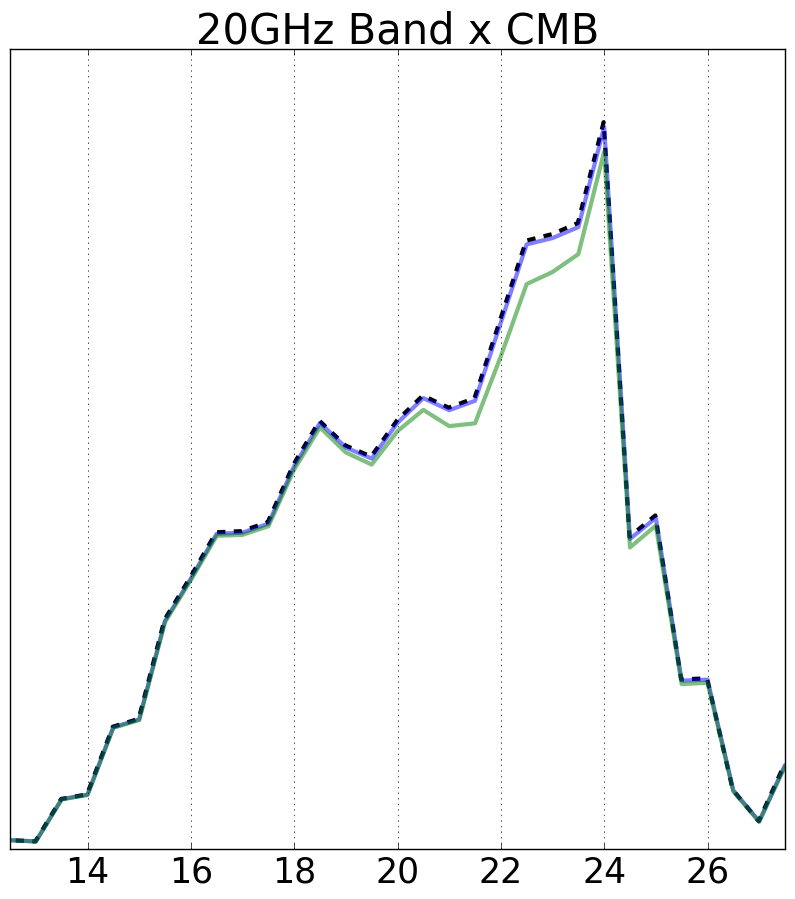
\includegraphics[width=.2\linewidth]{minmax_totals_20GHz_cmb.png}}
 \hspace{-2.5mm}
 \subfloat{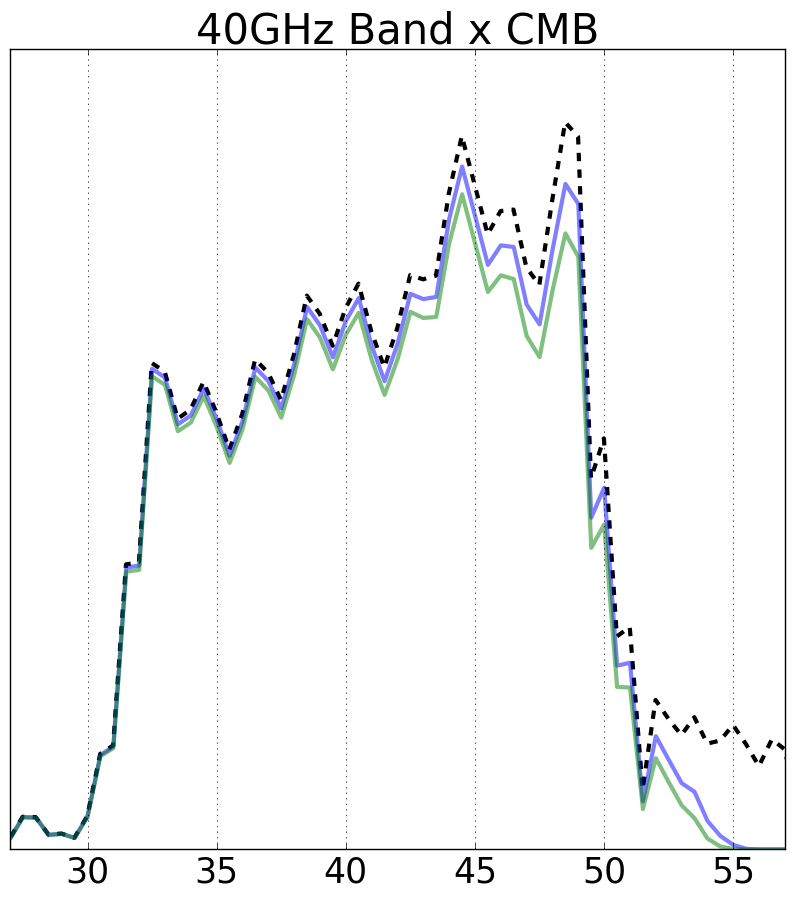
\includegraphics[width=.2\linewidth]{minmax_totals_40GHz_cmb.png}}
 \hspace{-2.5mm}
 \subfloat{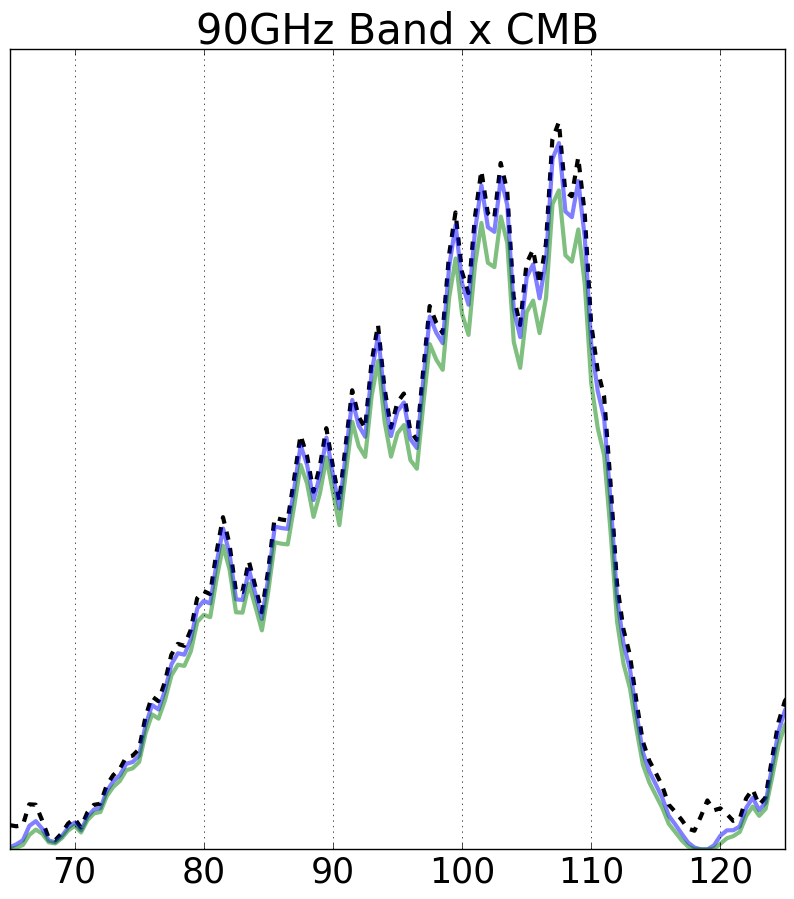
\includegraphics[width=.2\linewidth]{minmax_totals_90GHz_cmb.png}}
 \hspace{-2.5mm}
 \subfloat{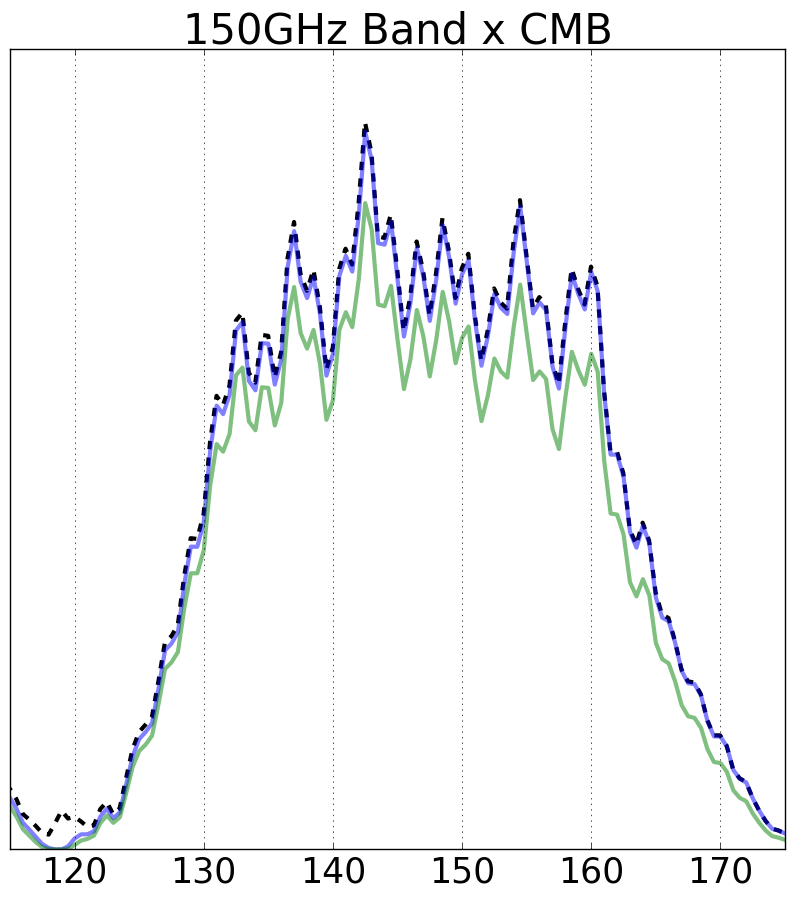
\includegraphics[width=.2\linewidth]{minmax_totals_150GHz_cmb.png}}
 \hspace{-2.5mm} 
 \subfloat{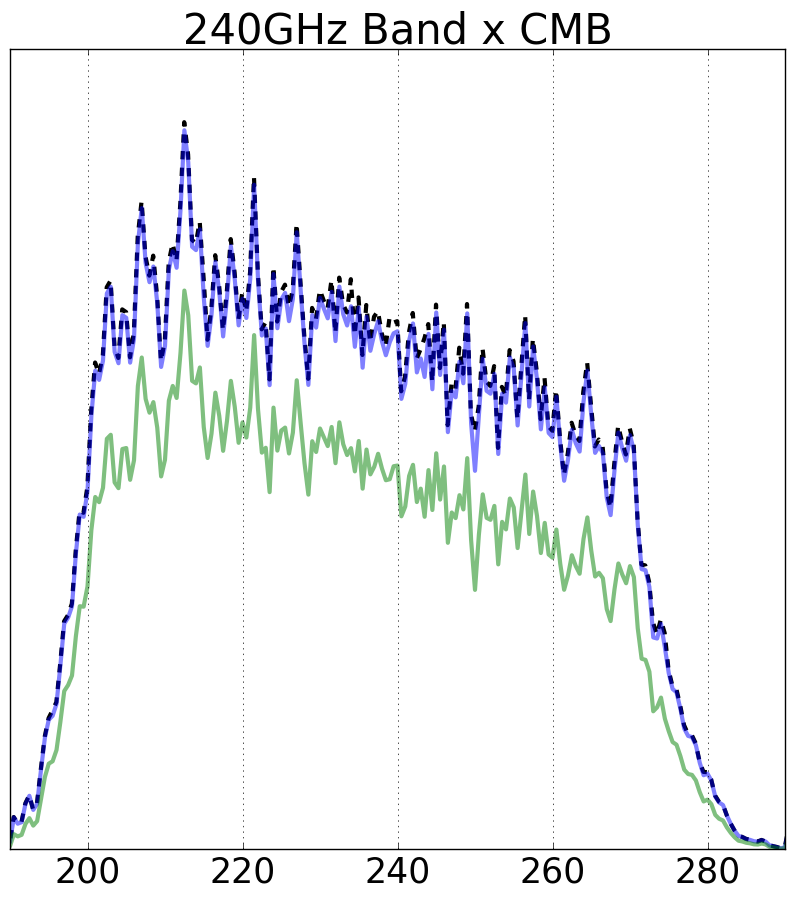
\includegraphics[width=.2\linewidth]{minmax_totals_240GHz_cmb.png}}
 \end{varwidth}
\caption{Minimum and maximum effects of the atmosphere for each of the five simulated frequency bands.  The top row shows the instrument band, the middle row shows band x dust, and the bottom row shows band x CMB.  The blue represents the minimum effect, the green represents the maximum effect, and the black dashed line shows the original band as measured by the FTS.  The y-axis of the plots goes from zero to one and represents the normalized transmission of the band, while the x-axis is the frequency in GHz.}
\label{minmax_bands}
\end{figure}

\FloatBarrier

\paragraph{Parameterization:}
Once all combinations of bands and transmission values are generated, the integrated power and band centers are solved for in each case.  To quantify the changes, we calculate the percent difference in the band gain and central frequency from the FTS measured band.  Tables \ref{minmax_gain} and \ref{minmax_center} outline the simulated changes in band gain and centers.  

\begin{table}[h]
 %\parbox{.25\linewidth}{
 \centering
 \resizebox{.5\linewidth}{!}{%
 \begin{tabular}{|c|l l|l l|l l|}
  \hline
  \multicolumn{7}{|c|}{Min and Max Percent Changes - Band Gain} \\
  \hline
  \multirow{3}{*}{Band} 
      & \multicolumn{2}{c|}{Band}
          & \multicolumn{2}{c|}{Dust}
              &\multicolumn{2}{c|}{CMB}\\             \cline{1-7}
  & Min & Max & Min & Max & Min & Max \\  \hline
   20GHz & 0.73\% & 3.22\% & 1.00\% & 4.08\% & 0.88\% & 3.77\% \\      
   40GHz & 4.24\% & 7.47\% & 5.83\% & 9.71\% & 5.07\% & 8.66\% \\      
   90GHz & 3.19\% & 8.98\% & 3.32\% & 9.35\% & 3.20\% & 9.04\% \\      
   150GHz & 1.41\% & 12.8\% & 1.33\% & 13.3\% & 1.40\% & 12.8\% \\      
   240GHz & 1.77\% & 27.8\% & 1.86\% & 28.6\% & 1.73\% & 27.45\% \\      \hline
 \end{tabular}}
\caption{Estimated minimum and maximum percent changes in band gain over a full observing season.}
\label{minmax_gain}
%}
%\hfill
%\parbox{.25\linewidth}{
\end{table}


\begin{table}
 \centering
 \resizebox{.5\linewidth}{!}{%
 \begin{tabular}{|c|l l|l l|l l|}
  \hline
  \multicolumn{7}{|c|}{Min and Max Percent Changes - Band Center} \\
  \hline
  \multirow{3}{*}{Band} 
      & \multicolumn{2}{c|}{Band}
          & \multicolumn{2}{c|}{Dust}
              &\multicolumn{2}{c|}{CMB}\\             \cline{1-7}
  & Min & Max & Min & Max & Min & Max \\  \hline
   20GHz & 0.03\% & 0.26\% & 0.07\% & 0.23\% & 0.05\% & 0.25\% \\      
   40GHz & 0.51\% & 0.78\% & 0.61\% & 0.89\% & 0.57\% & 0.85\% \\      
   90GHz & 0.01\% & 0.10\% & 0.08\% & 0.19\% & 0.03\% & 0.13\% \\      
   150GHz & -0.04\% & 0.20\% & -0.03\% & 0.24\% & -0.04\% & 0.20\% \\      
   240GHz & 0.02\% & 0.36\% & 0.02\% & 0.39\% & 0.02\% & 0.33\% \\      \hline
 \end{tabular}}
\caption{Estimated minimum and maximum percent changes in band center over a full observing season.}
\label{minmax_center}
%}
\end{table}

\FloatBarrier
